% Author: Izaak Neutelings (February 2023)
% Description: Signatures of long-lived particles
% Inspired by J. Antonelli in ICHEP 2016
%   https://indico.cern.ch/event/432527/contributions/1072042/attachments/1321320/1981614/Antonelli_ICHEP2016_CMSLLP.pdf
%   https://twiki.cern.ch/twiki/bin/view/CMS/ExoticaLongLived (CMS internal)
% Sources:
%   CMS Silicon detector: https://cms.cern/detector/identifying-tracks/silicon-strips
%   LLPs: https://royalsocietypublishing.org/doi/10.1098/rsta.2019.0047
%   LLPs: https://hrussell.web.cern.ch/hrussell/graphics.html
%   LLPs: https://indico.cern.ch/event/607314/contributions/2542309/attachments/1447873/2231444/20170424_LLPs.pdf
\documentclass[border=3pt,tikz]{standalone}
\usepackage{amsmath}
\usetikzlibrary{calc}
\usetikzlibrary{math} % for \tikzmath
\usetikzlibrary{decorations.pathmorphing} % for snake, coil, zigzag
\tikzset{>=latex} % set default arrow head as latex

% COLORS
\colorlet{leptoncol}{green!70!black}
\colorlet{quarkcol}{blue!85!cyan!80!black}
\colorlet{photoncol}{yellow!80!orange!90!black}
\colorlet{exocol}{red!80!black}
\colorlet{anycol}{blue!80!cyan!60!red!95!black!90}

% STYLES
\tikzstyle{label}=[align=center,rounded corners=3pt] %fill=blue!60!cyan!80!black!15,
\tikzstyle{legend}=[draw=black,thick,rounded corners=3pt] %,fill=blue!60!cyan!80!black!15
\tikzstyle{entry}=[right=1pt,inner sep=4pt]
\tikzstyle{particle}=[anycol,very thick,line cap=round]
\tikzstyle{lepton}=[particle,leptoncol]
\tikzstyle{quark}=[particle,quarkcol]
\tikzstyle{track}=[quark,thick]
\tikzstyle{photon}=[particle,photoncol,decorate,decoration={
  snake,amplitude=.4mm,segment length=2.5mm,post length=1mm}]
\tikzstyle{charged exo}=[particle,exocol]
\tikzstyle{neutral exo}=[charged exo,dashed]

% JET CONE
\newcommand\jetcone[6][quarkcol]{{
  \pgfmathanglebetweenpoints{\pgfpointanchor{#2}{center}}{\pgfpointanchor{#3}{center}}
  \pgfmathsetmacro\oang{#4/2} % half-opening angle
  \edef\e{#5} % ratio a/b ("eccentricity") of cone top
  \def\tmpL{tmpL-#2-#3} % unique coordinate name
  \edef\vang{\pgfmathresult} % angle of vector OV
  \tikzmath{
    coordinate \C;
    \C = (#2)-(#3); % vector OV
    \x = veclen(\Cx,\Cy)*\e*sin(\oang)^2; % x coordinate P
    \y = tan(\oang)*(veclen(\Cx,\Cy)-\x); % y coordinate P
    \a = veclen(\Cx,\Cy)*sqrt(\e)*sin(\oang); % vertical radius
    \b = veclen(\Cx,\Cy)*tan(\oang)*sqrt(1-\e*sin(\oang)^2); % horizontal radius
    \angb = acos(sqrt(\e)*sin(\oang)); % angle of P in ellipse
  }
  \coordinate (#2-v) at ($(#2)+(\vang:1pt)$); % shift vertex
  \coordinate (\tmpL) at ($(#3)-(\vang:\x pt)+(\vang+90:\y pt)$); % tangency
  \draw[thin,#1!50!black,fill=#1!80!black!50,line cap=round,rotate=\vang] % cone back
    (#2) -- (\tmpL) arc(180-\angb:180+\angb:{\a pt} and {\b pt}) -- (#2); %-- cycle;
  \draw[thin,#1!50!black,rotate=\vang, % cone inside
        top color=#1!60!black!60,bottom color=#1!50!black!75,shading angle=\vang]
    (#3) ellipse({\a pt} and {\b pt});
  #6 % extra tracks
  \draw[thin,#1!50!black,rotate=\vang,fill opacity=0.80, % cone front
        top color=#1!90!black!20,bottom color=#1!50!black!50,line cap=round,shading angle=\vang]
    (#2) -- (\tmpL) arc(180-\angb:180+\angb:{\a pt} and {\b pt}) -- (#2); %-- cycle;
}}

% DETECTOR
\def\scale{1.6} % scale diagrams
\def\keepseg#1#2{% % return boolean if detector segment falls outside mask
  (\mask==0 || (#2>\angmin-4 && #1<\angmax+4) || (#2>\angmin+356 && #1<\angmax+364))
}
\tikzset{
  pics/detector/.style args={#1:#2}{
    code={
  
  % MASK except segment
  \pgfmathsetmacro\mask{#1!=#2}
  \pgfmathsetmacro\angmin{#1>=0 ? #1 : 360+#1}
  \pgfmathsetmacro\angmax{#2>=0 ? #2 : 360+#2}
  \message{^^JDetector: 1=#1, 2=#2, angmin=\angmin, angmax=\angmax, mask=\mask}
  \begin{scope}[pic actions]
  
  % CLIP
  \ifnum\mask=1 % clip detector segment
    %\draw[thick,black] (0,0) -- (#1:2.3) arc(#1:#2:2.3) -- cycle;
    %\clip (0,0) -- (\angmin:2.3) arc(\angmin:\angmax:2.3) -- cycle;
    \clip (0,0) -- (#1:2.3) arc(#1:#2:2.3) -- cycle;
  \fi
  
  % PIXEL TRACKER (PBIX)
  \foreach \Rlay in {0.09,0.13,0.17,0.21}{
    \message{^^JPixel tracker: Rlay=\Rlay}
    \draw[line width=0.1] (0,0) circle(\Rlay);
  }
  
  % SILICON INNER TRACKER (TIB)
  \def\h{0.12}
  \def\w{0.010}
  \def\d{0.028}
  \foreach \Rlay/\Nlay in {0.40/30,0.55/38,0.70/46,0.85/52}{
    \message{^^JInner tracker: Rlay=\Rlay, Nlay=\Nlay}
    \foreach \i [
      evaluate={\ang=\i*(360/\Nlay);\keep=\keepseg{\ang}{\ang};}
    ] in {1,...,\Nlay}{
      \ifnum\keep=1
        \fill[rotate around={\ang+10:(\ang:\Rlay-\d)},rounded corners=0.05pt]
          (\ang:\Rlay-\d)++(-\w/2,-\h/2) rectangle++(\w,\h);
        \fill[rotate around={\ang+10:(\ang:\Rlay+\d)},rounded corners=0.05pt]
          (\ang:\Rlay+\d)++(-\w/2,-\h/2) rectangle++(\w,\h);
      \fi
    }
  }
  
  % OUTER TRACKER (TOB)
  \def\h{0.18}
  \def\w{0.011}
  \def\d{0.021}
  \foreach \Rlay/\Nlay in {1.00/21,1.12/24,1.24/27,1.36/30,1.48/33,1.64/37}{
    \message{^^JOuter tracker: Rlay=\Rlay, Nlay=\Nlay}
    \foreach \i [
      evaluate={\anga=(\i-1)*360/\Nlay;\angb=(\i-0.5)*360/\Nlay;
                \keep=\keepseg{\anga}{\angb};}
    ] in {1,...,\Nlay}{
      \ifnum\keep=1
        \fill[rotate={\anga},rounded corners=0.05pt]
          (0:\Rlay-\d-0.55*\w)++(-\w/2,-\h/2) rectangle++(\w,\h)
          (0:\Rlay-\d+0.55*\w)++(-\w/2,-\h/2) rectangle++(\w,\h);
        \fill[rotate={\angb},rounded corners=0.1pt]
          (0:\Rlay+\d-0.55*\w)++(-\w/2,-\h/2) rectangle++(\w,\h)
          (0:\Rlay+\d+0.55*\w)++(-\w/2,-\h/2) rectangle++(\w,\h);
      \fi
    }
  }
  
  % ECAL
  \def\Ntow{18}
  \def\Rin{1.85} % inner radius
  \def\Rout{2.24} % outer radius
  \message{^^JECAL: Ntow=\Ntow}
  \foreach \i [
      evaluate={\anga=(\i-1.5)*360/\Ntow;\angb=(\i-0.5)*360/\Ntow;
                \keep=\keepseg{\anga}{\angb};}
    ] in {1,...,\Ntow}{
      \ifnum\keep=1
        \draw (\anga:\Rin) -- (\anga:\Rout) --
              (\angb:\Rout) -- (\angb:\Rin) -- cycle;
      \fi
  }
  
  %% HCAL
  %\def\Rin{2.28} % inner radius
  %\def\Rout{3.8} % outer radius
  %\message{^^JHCAL: Ntow=\Ntow}
  %\foreach \i [
  %    evaluate={\anga=(\i-1.5)*360/\Ntow;\angb=(\i-0.5)*360/\Ntow;}
  %  ] in {1,...,\Ntow}{
  %  \draw
  %    (\anga:\Rin) -- (\anga:\Rout) --
  %    (\angb:\Rout) -- (\angb:\Rin) -- cycle;
  %}
  
  \end{scope}
  \ifnum\mask=1
    \draw[black!30] (\angmax:2.5) -- (0,0) -- (\angmin:2.5);
  \fi
    
    }
  },
  pics/detector/.default={0:0}
}

\begin{document}


% LLP SIGNATURES in the CMS detector
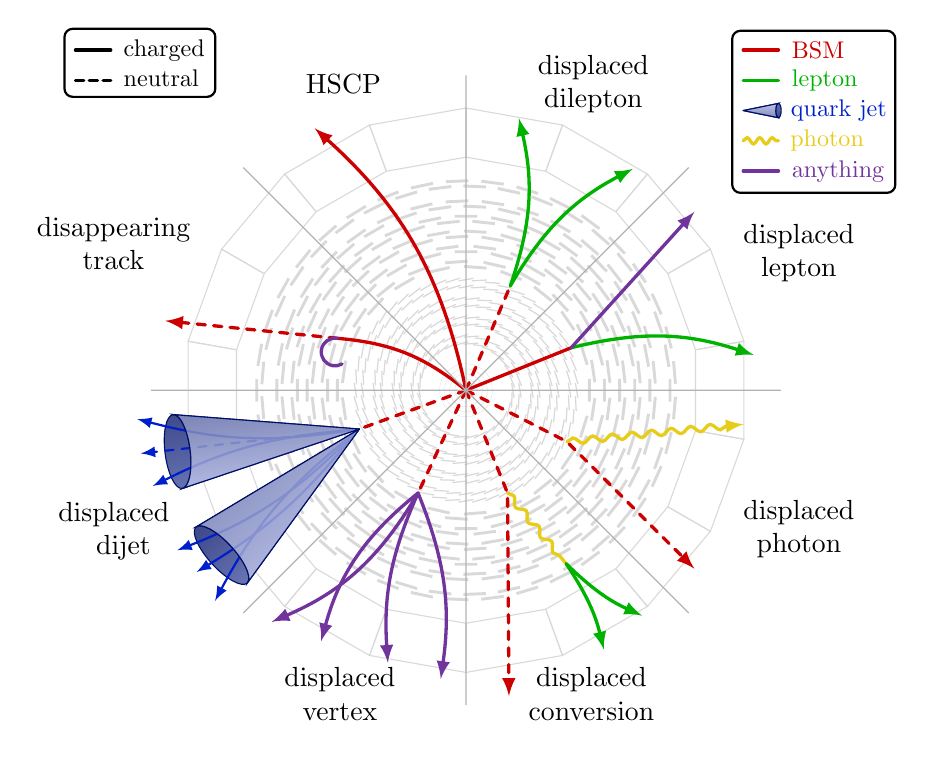
\begin{tikzpicture}[scale=\scale]
  %\def\R{2} % tracker outer radius
  %\def\dang{4} % angular granularity of calo deposits, CMS: 0.0175*180/pi = 1
  %% HELP GRID
  %\draw[black!20,opacity=0.2,very thin]
  %  \foreach \r in {0.2,0.4,...,4.4}{(0,0) circle(\r)}
  %  \foreach \a in {0,10,...,350}{(0,0) -- (\a:4.4)};
  %\draw[black!40,opacity=0.2,thin]
  %  \foreach \r in {1,...,4}{(0,0) circle(\r)}
  %  \foreach \a in {0,30,...,330}{(0,0) -- (\a:4.4)};
  
  % DETECTOR
  \pic[black!15,scale=\scale] {detector};
  
  % DISPLACED LEPTON
  \message{^^JParticles}
  \draw[charged exo] (0,0) -- (22:0.90) coordinate (V);
  \draw[->,lepton] (V) to[bend left=16] (7:2.3);
  \draw[->,particle] (V) -- (38:2.3);
  
  % DISPLACED DILEPTON
  \draw[neutral exo] (0,0) -- (67:0.90) coordinate (V);
  \draw[->,lepton] (V) to[bend left=16] (53:2.2);
  \draw[->,lepton] (V) to[bend right=16] (79:2.2);
  
  % HSCP
  \draw[->,charged exo] (0,0) to[bend right=18] (120:2.4);
  
  % DISAPPEARING TRACK
  \draw[charged exo] (0,0) to[bend right=17] (158:1.1) coordinate (V);
  \draw[->,neutral exo] (V) -- (167:2.45);
  \draw[particle] (V) arc(80:300:0.11);
  
  % DISPLACED JET
  \draw[neutral exo] (0,0) -- (-160:0.90) coordinate (V);
  %\draw[->,quark] (V) to[bend left=16] (-172:2.45);
  %\draw[->,quark] (V) to[bend right=16] (-148:2.45);
  \coordinate (J1) at (-168:2.34); % jet 1 vector
  \coordinate (J2) at (-146:2.34); % jet 2 vector
  \jetcone[quarkcol]{V}{J1}{23}{0.12}{ % jet 1
    \draw[->,track] (V-v) to[bend left=12] (-175:2.62);
    \draw[->,track] (V-v) to[bend right=11] (-163:2.60);
    \draw[->,track,dashed] (V-v) -- (-169:2.63);
  }
  \jetcone[quarkcol]{V}{J2}{23}{0.12}{ % jet 2
    \draw[->,track] (V-v) to[bend right=12] (-140:2.60);
    \draw[->,track] (V-v) to[bend left=10] (-146:2.58);
    \draw[->,track] (V-v) to[bend left=12] (-151:2.62);
  }
  
  % DISPLACED VERTEX
  \draw[neutral exo] (0,0) -- (-115:0.90) coordinate (V);
  \draw[->,particle] (V) to[bend left=18] (-130:2.4);
  \draw[->,particle] (V) to[bend right=18] (-120:2.3);
  \draw[->,particle] (V) to[bend right=14] (-106:2.25);
  \draw[->,particle] (V) to[bend left=15] (-95:2.3);
  
  % DISPLACED CONVERSION
  \draw[->,neutral exo]
    (0,0) -- (-68:0.88) coordinate (V) -- (-82:2.45);
  \draw[photon] (V) -- (-60:1.59) coordinate (P);
  \draw[->,lepton] (P) to[bend right=10] (-52:2.27);
  \draw[->,lepton] (P) to[bend left=10] (-62:2.33);
  
  % DISPLACED PHOTON
  \draw[->,neutral exo]
    (0,0) -- (-27:0.90) coordinate (V) -- (-38:2.3);
  \draw[->,photon] (V) -- (-7:2.22);
  
  % CHARGE LEGEND
  \def\lw{0.28} % legend length
  \def\lh{0.24} % legend line spacing
  \begin{scope}[shift={(-3.1,2.7)},every node/.style={scale=0.87,thick}]
    \draw[particle,black]
      (0,0) -- (\lw,0) node[entry] (A) {charged}; %particle
    \draw[particle,densely dashed,black]
      (0,-\lh) -- (\lw,-\lh) node[yshift=1pt,entry] (B) {neutral}; %particle
    \draw[legend] (B.south west)++(-1.38*\lw,0) rectangle (A.north east);
  \end{scope}
  
  % COLOR LEGEND
  \begin{scope}[shift={(2.2,2.7)},every node/.style={scale=0.87}]
    \coordinate (JA) at (0,-2*\lh);
    \coordinate (JB) at (\lw,-2*\lh);
    \draw[charged exo] (0,0) -- (\lw,0) node[entry] (A) {BSM};
    \draw[lepton] (0,-\lh) -- (\lw,-\lh) node[entry] {lepton};
    %\draw[quark] (0,-2*\lh) -- (\lw,-2*\lh) node[entry] {quark};
    \jetcone[quarkcol]{JA}{JB}{23}{0.15}{}
    \node[entry,quarkcol] at (JB) {quark jet};
    \draw[photon,decoration={segment length=1.6mm,post length=0mm}]
      (0,-3*\lh) -- (\lw,-3*\lh) node[right=1pt] {photon};
    \draw[particle] (0,-4*\lh) -- (\lw,-4*\lh) node[entry] (B) {anything};
    \draw[legend] (A.north west)++(-1.38*\lw,0) rectangle (B.south east);
  \end{scope}
  
  % LABELS
  \def\Nlab{8}
  \def\Rlab{2.3}
  \draw[black!30] \foreach \a in {0,45,...,360}{(0,0) -- (\a:2.5)};
  %\node[align=center] at (112.5:\Rlab) {HSCP};
  %\node[align=center] at (67.5:\Rlab) {displaced\\dilepton};
  \foreach \lab [%
    count=\i,evaluate={\ang=(\i-0.5)*360/8;}
  ] in {%
    displaced\\lepton,displaced\\dilepton,HSCP\\[-5pt],
    disappearing\\track,displaced\hspace*{7pt}\\dijet,displaced\\vertex,
    displaced\\conversion,displaced\\photon%
  }{
    \node[label,anchor={\ang+180}] %,font=\bf]
      at (\ang:\Rlab) {\lab};
  }
  
\end{tikzpicture}


%% LLP SIGNATURE: DISPLACED LEPTON
%\begin{tikzpicture}[scale=\scale,rotate=180]
%  \draw pic[black!15,scale=\scale] {detector={180:225}};
%  \draw[charged exo] (0,0) -- (22:0.90) coordinate (V);
%  \draw[->,lepton] (V) to[bend left=16] (7:2.3);
%  \draw[->,particle] (V) -- (38:2.3);
%\end{tikzpicture}
%
%
%% LLP SIGNATURE: DISPLACED DILEPTON
%\begin{tikzpicture}[scale=\scale,rotate=135]
%  \draw pic[black!15,scale=\scale] {detector={180:225}};
%  \draw[neutral exo] (0,0) -- (67:0.90) coordinate (V);
%  \draw[->,lepton] (V) to[bend left=16] (53:2.2);
%  \draw[->,lepton] (V) to[bend right=16] (79:2.2);
%\end{tikzpicture}
%
%
%% LLP SIGNATURE: HSCP
%\begin{tikzpicture}[scale=\scale,rotate=90]
%  \draw pic[black!15,scale=\scale] {detector={180:225}};
%  \draw[->,charged exo] (0,0) to[bend right=18] (120:2.4);
%\end{tikzpicture}
%
%
%% LLP SIGNATURE: DISAPPEARING TRACK
%\begin{tikzpicture}[scale=\scale,rotate=45]
%  \draw pic[black!15,scale=\scale] {detector={180:225}};
%  \draw[charged exo] (0,0) to[bend right=17] (158:1.1) coordinate (V);
%  \draw[->,neutral exo] (V) -- (167:2.45);
%  \draw[lepton] (V) arc(80:300:0.11);
%\end{tikzpicture}
%
%
%% LLP SIGNATURE: DISPLACED JETS
%\begin{tikzpicture}[scale=\scale,rotate=0]
%  \draw pic[black!15,scale=\scale] {detector={180:225}};
%  \draw[neutral exo] (0,0) -- (-160:0.90) coordinate (V);
%  %\draw[->,quark] (V) to[bend left=16] (-172:2.45);
%  %\draw[->,quark] (V) to[bend right=16] (-148:2.45);
%  \coordinate (J1) at (-168:2.34); % jet 1 vector
%  \coordinate (J2) at (-146:2.34); % jet 2 vector
%  \jetcone[quarkcol]{V}{J1}{23}{0.12}{ % jet 1
%    \draw[->,track] (V-v) to[bend left=12] (-175:2.62);
%    \draw[->,track] (V-v) to[bend right=11] (-163:2.60);
%    \draw[->,track,dashed] (V-v) -- (-169:2.63);
%  }
%  \jetcone[quarkcol]{V}{J2}{23}{0.12}{ % jet 2
%    \draw[->,track] (V-v) to[bend right=12] (-140:2.60);
%    \draw[->,track] (V-v) to[bend left=10] (-146:2.58);
%    \draw[->,track] (V-v) to[bend left=12] (-151:2.62);
%  }
%\end{tikzpicture}
%
%
%% LLP SIGNATURE: DISPLACED VERTEX
%\begin{tikzpicture}[scale=\scale,rotate=-45]
%  \draw pic[black!15,scale=\scale] {detector={180:225}};
%  \draw[neutral exo] (0,0) -- (-115:0.90) coordinate (V);
%  \draw[->,particle] (V) to[bend left=18] (-130:2.4);
%  \draw[->,particle] (V) to[bend right=18] (-120:2.3);
%  \draw[->,particle] (V) to[bend right=14] (-106:2.25);
%  \draw[->,particle] (V) to[bend left=15] (-95:2.3);
%\end{tikzpicture}
%
%
%% LLP SIGNATURE: DISPLACED CONVERSION
%\begin{tikzpicture}[scale=\scale,rotate=-90]
%  \draw pic[black!15,scale=\scale] {detector={180:225}};
%  \draw[->,neutral exo]
%    (0,0) -- (-68:0.88) coordinate (V) -- (-82:2.45);
%  \draw[photon] (V) -- (-60:1.59) coordinate (P);
%  \draw[->,lepton] (P) to[bend right=10] (-52:2.27);
%  \draw[->,lepton] (P) to[bend left=10] (-62:2.33);
%\end{tikzpicture}
%
%
%% LLP SIGNATURE: DISPLACED PHOTON
%\begin{tikzpicture}[scale=\scale,rotate=-135]
%  \draw pic[black!15,scale=\scale] {detector={180:225}};
%  \draw[->,neutral exo]
%    (0,0) -- (-27:0.90) coordinate (V) -- (-38:2.3);
%  \draw[->,photon] (V) -- (-7:2.22);
%\end{tikzpicture}
%
%
%% FOR LOOP: Make HNL diagrams with quarter and full tracker
%\foreach \dang [evaluate={\lang=(\dang>200?-102:-23);}] in {270,180}{
%
%% LLP SIGNATURE: DISPLACED DILEPTON + PROMPT LEPTON
%% E.g. a heavy neutral lepton (HNL)
%\begin{tikzpicture}[scale=\scale,rotate=0]
%  \def\angN{-164} % angle of HNL
%  \draw pic[black!15,scale=\scale] {detector={180:\dang}};
%  \coordinate (PV) at (0,0); % primary vertex
%  \draw[neutral exo] (PV) -- (\angN:0.90) coordinate (V)
%    node[pos=0.7,above=0pt] {N};
%  \coordinate (L1) at (\lang:2.50); % prompt lepton
%  \coordinate (L2) at (\angN+20:2.42); % displaced lepton 1
%  \coordinate (L3) at (\angN-9:2.42); % displaced lepton 2
%  \coordinate (N) at (\angN+4:2.42); % displaced neutrino
%  \draw[->,lepton] (PV) to[bend right=11] (L1) % prompt lepton
%    node[anchor=172+\lang,inner sep=1pt] {$\ell_1$};
%  \draw[->,lepton] (V) to[bend right=16] (L2) % displaced lepton 1
%    node[anchor=40,inner sep=1pt] {$\ell_2$};
%  \draw[->,lepton] (V) to[bend left=16] (L3) % displaced lepton 2
%    node[anchor=20,inner sep=1pt] {$\ell_3$};
%  \draw[->,lepton,dashed] (V) -- (N) % displaced neutrino
%    node[anchor=40,inner sep=1pt] {$\nu$};
%\end{tikzpicture}
%
%% LLP SIGNATURE: DISPLACED JET + PROMPT LEPTON
%% E.g. a heavy neutral lepton (HNL)
%\begin{tikzpicture}[scale=\scale,rotate=0]
%  \def\angN{-162} % angle of HNL
%  \draw pic[black!15,scale=\scale] {detector={180:\dang}};
%  \coordinate (PV) at (0,0); % primary vertex
%  \draw[neutral exo] (PV) -- (\angN:0.90) coordinate (V)
%    node[pos=0.7,above=0pt] {N};
%  \coordinate (J) at (\angN-2:2.34); % displaced jet vector
%  \coordinate (L1) at (\lang:2.50); % prompt lepton
%  \coordinate (L2) at (\angN+19:2.42); % displaced lepton
%  \draw[->,lepton] (PV) to[bend right=11] (L1) % prompt lepton
%    node[anchor=172+\lang,inner sep=1pt] {$\ell_1$};
%  \draw[->,lepton] (V) to[bend left=16] (L2) % displaced lepton
%    node[anchor=40,inner sep=1pt] {$\ell_2$};
%  \jetcone[quarkcol]{V}{J}{23}{0.12}{ % displaced jet
%    \draw[->,track] (V-v) to[bend left=12] (\angN-9:2.62);
%    \draw[->,track] (V-v) to[bend right=11] (\angN+4:2.60);
%    \draw[->,track,dashed] (V-v) -- (\angN-3:2.63);
%  }
%\end{tikzpicture}
%
%% LLP SIGNATURE: DISPLACED JET + PROMPT LEPTON (boosted)
%% E.g. a heavy neutral lepton (HNL), boosted N -> lqq'
%\begin{tikzpicture}[scale=\scale,rotate=0]
%  \def\angN{-162} % angle of HNL
%  \draw pic[black!15,scale=\scale] {detector={180:\dang}};
%  \coordinate (PV) at (0,0); % primary vertex
%  \draw[neutral exo] (PV) -- (\angN:0.90) coordinate (V)
%    node[pos=0.7,above=0pt] {N};
%  \coordinate (J) at (\angN-2:2.34); % displaced jet vector
%  \coordinate (L1) at (\lang:2.50); % prompt lepton
%  \coordinate (L2) at (\angN+5:2.69); % displaced lepton
%  \draw[->,lepton] (PV) to[bend right=13] (L1) % prompt lepton
%    node[anchor=172+\lang,inner sep=1pt] {$\ell_1$};
%  \jetcone[quarkcol]{V}{J}{23}{0.12}{ % displaced jet
%    \draw[->,track] (V-v) to[bend left=12] (\angN-9:2.62);
%    \draw[->,track] (V-v) to[bend right=11] (\angN+1:2.60);
%    \draw[->,track,dashed] (V-v) -- (\angN-3:2.63);
%    \draw[->,lepton] (V-v) to[bend right=14] (L2) % displaced lepton
%      node[anchor=40,inner sep=0pt] {$\ell_2$};
%  }
%\end{tikzpicture}
%
%} % end \foreach


\end{document}